\chapter{Geometry}

\section{Basics}

A determinant of a $2x2$ matrix is defined as
\[
    \left\vert
        \begin{array}{cc}
            a & b \\
            c & d \\
        \end{array}
    \right\vert
    = a d - b c
\]

\section{java.awt.geom}

The \texttt{java.awt.geom} and \texttt{java.awt} packages have, albeit limited, facilities
for geometric problems.  There are classes to represent shapes - see
\href{http://docs.oracle.com/javase/6/docs/api/java/awt/Shape.html}{java.awt.Shape}, including
lines, ellipses, rectangles and some curves.

\begin{itemize}
\item "is contained in".  java.awt.geom.Shape provide a contains() method to test if a point
    is contained in a shape.  Contains() returns true if the point is in the interior, and false
    if the point is outside the shape. However, it \textbf{may return true or false if the point is 
    on the shape boundary.} 

\begin{figure}
    \centering
    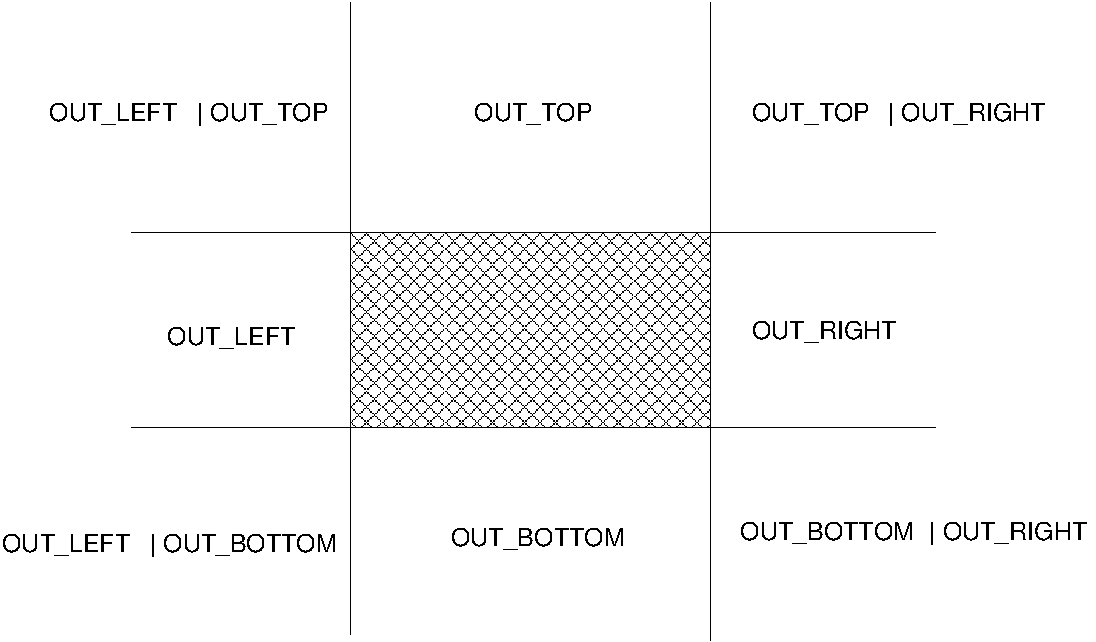
\includegraphics[height=2in]{outcode.pdf}
    \caption{Outcode - note that points that lie on any of the sidelines are considered inside.}
    \label{fig:outcode}
\end{figure}

\item "outcode". Outcodes were invented by Cohen-Sutherland; they are used for clipping
    in computer graphics.  java.awt.geom.Rectangle2D provides an outcode() method.
    The result is 0 if a point is inside or on any sideline of the rectangle; otherwise 
    the result is a
    combination of bits that represent where the point lies in relationship to the
    rectangle, as shown in Figure~\ref{fig:outcode}.
    For clipping of lines, the outcodes of the start and end point are
    computed, which then allows a quick identification of whether the line is inside,
    must be clipped, may be ignored, or needs further investigation.
    A useful property of outcode() is that it can substitute as a replacement for
    contains() in case where a point may lie on an edge but should be considered
    inside. 

\item "intersects."  Tests if a shape intersects with a rectangle.
    Can also test if two lines or line segments intersect, but cannot find the point of
    intersection.

\item "is point on line segment." Implements this as Line2D.ptSegDistSq(Point2D) $<$ 1e-9.

\end{itemize}

\section{Coordinate Geometry}

\subsection{Line/Line Intersection}
\label{sec:lineintersection}
\index{Line/Line Intersections}

\begin{figure}
    \centering
    % Wikipedia Public Domain image
    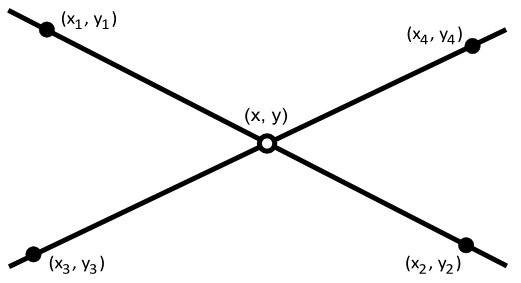
\includegraphics[height=1.5in]{Line-Line_Intersection.png}
    \caption{Line line intersection}
    \label{fig:linelineintersect}
\end{figure}

\[
\begin{array}{ll}
P_x = \frac{\begin{vmatrix} 
                \begin{vmatrix} x_1 & y_1\\
                                x_2 & y_2
                \end{vmatrix} & 
                \begin{vmatrix} x_1 & 1\\
                                x_2 & 1
                \end{vmatrix} \\\\ 
                \begin{vmatrix} x_3 & y_3\\
                                x_4 & y_4
                \end{vmatrix} & 
                \begin{vmatrix} x_3 & 1\\
                                x_4 & 1
                \end{vmatrix} 
            \end{vmatrix} }{
            \begin{vmatrix} 
                \begin{vmatrix} x_1 & 1\\
                               x_2 & 1
                \end{vmatrix} &  
                \begin{vmatrix} y_1 & 1\\
                                y_2 & 1
             \end{vmatrix} \\\\ 
             \begin{vmatrix} x_3 & 1\\
                             x_4 & 1
             \end{vmatrix} & 
             \begin{vmatrix} y_3 & 1\\
                             y_4 & 1 
             \end{vmatrix} 
            \end{vmatrix}}

&

P_y = \frac{\begin{vmatrix} 
                \begin{vmatrix} x_1 & y_1\\
                                x_2 & y_2
                \end{vmatrix} &  
                \begin{vmatrix} y_1 & 1
                              \\y_2 & 1
                \end{vmatrix} \\\\ 
                \begin{vmatrix} x_3 & y_3\\
                                x_4 & y_4
                \end{vmatrix} & 
                \begin{vmatrix} y_3 & 1\\
                                y_4 & 1
                \end{vmatrix} 
            \end{vmatrix} }
           {\begin{vmatrix} 
               \begin{vmatrix} x_1 & 1\\
                               x_2 & 1
               \end{vmatrix} &
               \begin{vmatrix} y_1 & 1\\
                               y_2 & 1
            \end{vmatrix} \\\\ 
            \begin{vmatrix} x_3 & 1\\
                            x_4 & 1
            \end{vmatrix} & 
            \begin{vmatrix} y_3 & 1\\
                            y_4 & 1
            \end{vmatrix} 
     \end{vmatrix}}\,\!
\\

\end{array}
\]

The determinants can be written out as:
\begin{align*}
    (P_x, P_y)= \bigg(&\frac{(x_1 y_2-y_1 x_2)(x_3-x_4)-(x_1-x_2)(x_3 y_4-y_3 x_4)}{(x_1-x_2)(y_3-y_4)-(y_1-y_2)(x_3-x_4)}, \\
                      &\frac{(x_1 y_2-y_1 x_2)(y_3-y_4)-(y_1-y_2)(x_3 y_4-y_3 x_4)}{(x_1-x_2)(y_3-y_4)-(y_1-y_2)(x_3-x_4)}\bigg)
\end{align*}

Source: \href{http://en.wikipedia.org/wiki/Line-line_intersection}{http://en.wikipedia.org/wiki/Line-line\_intersection}.

\paragraph{Notes}
\begin{itemize}
\item Does not handle parallel or coincident lines:
    Denominator will be zero:
    \[
        (x_1 - x_2) (y_3 - y_4) - (y_1 - y_2) (x_3 - x_4) = 0
    \]
\item Does not handle if lines are each others' normal (i.e., at a right angle).
    If line is horizontal ($y_1 = y_2$ or $y_3 = y_4$), and the other vertical ($x_1 = x_2$ or $x_3 = x_4$) 
    denominator will also be a 0 determinant, but the lines will intersect.  
    Handle as special case if problem allows it.

\item Intersection point may be outside the given segments.

\item If you only need to know if two lines intersect, but not where, use java.awt.geom.Line2D.intersects.
\end{itemize}

\paragraph{Code}

This code is from a solution to 2011/F (Section~\ref{sec:2011-f-lineofsight}) where the 
parallel and rectangular cases do not occur. (TBD: provide complete implementation.)

\inputminted[fontsize=\footnotesize,linenos=true]{java}{code/lineintersection.java}

%
%
%

\subsection{Area of a Polygon}
\label{sec:areapolygon}
\index{Polygon!Area}
\index{Area!Polygon}
\index{Polygon}

The signed area of a planar non-self-intersecting polygon with vertices $(x_1, y_1), \dots, (x_n, y_n)$ is
\[
    A = \frac{1}{2} \left(
        \left\vert
        \begin{array}{cc}
            x_1 & x_2 \\
            y_1 & y_2 \\
        \end{array}
        \right\vert
        +
        \left\vert
        \begin{array}{cc}
            x_2 & x_3 \\
            y_2 & y_3 \\
        \end{array}
        \right\vert
        + \ldots +
        \left\vert
        \begin{array}{cc}
            x_n & x_1 \\
            y_n & y_1 \\
        \end{array}
        \right\vert
        \right)
\]

Figure~\ref{fig:polygonareadeterminant} shows how to multiply this out
\[
    A = \frac{1}{2} \left(
        x_1 y_2 - x_2 y_1
      + x_2 y_3 - x_3 y_2
      + \ldots +
      + x_{n-1} y_n - x_n y_{n-1}
      + x_{n} y_1 - x_1 y_n
      \right)
\]

(Source: Mathworld~\cite{mathworldpolygonarea})

\begin{figure}
    \centering
    % Wikipedia Public Domain image
    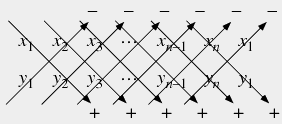
\includegraphics[height=1.5in]{PolygonArea_1000.png}
    \caption{Line line intersection}
    \label{fig:polygonareadeterminant}
\end{figure}

\paragraph{Notes}
\begin{itemize}
\item Works for any simple polygon (concave or convex)
\item Does not work for complex polygons (when any edges intersect)
\item Points \textbf{must be ordered} if polygon has more than 3 vertices, or output is junk.
\item A is positive if points are in counterclockwise order, negative if points are in clockwise order.
    See the use of Math.abs() in code below.
\item Triangle and any Quadrilateral are, of course, just special cases.
    For triangles, order does not matter.
\end{itemize}

\paragraph{Code}
\inputminted[fontsize=\footnotesize,linenos=true]{java}{code/polygonarea.java}

Special case of a triangle:

\inputminted[fontsize=\footnotesize,linenos=true]{java}{code/triangleareacoord.java}

%%%%%%%%%%%%%%%%%%%%%%%%%%%%%%%%%%%%%%%%%%%%%%%%%%%%%%%%%%%%%%%%%%%%%%%%%%%%%%%%%%%%%%%%%%%
%
%
\subsection{Convex Hull}
\label{sec:convexhull}
\index{Polygon!Convex Hull}
\index{Convex Hull}

A frequent favorite is the computation of the convex hull of a set of points in the plane,
defined as the smallest convex polygon that encloses all points.

\begin{figure}
    \centering
    % Wikipedia Public Domain image
    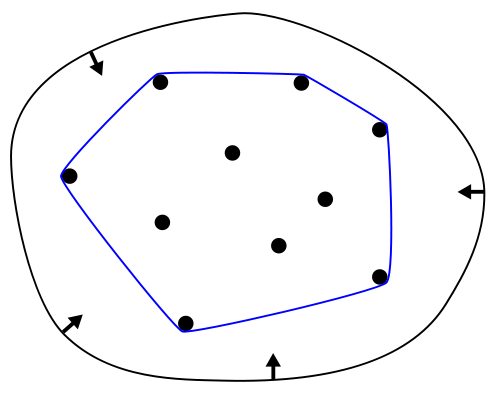
\includegraphics[height=2in]{500px-ConvexHull.png}
    \caption{Convex Hull - Rubber Band analogy. The convex hull is the convex polygon created 
        when spanning a rubber band around a set of points.}
    \label{fig:convexhull}
\end{figure}

